\section{Introduction}
In the past decade, with the introduction of technology that can store huge amounts of data, a large amount of musical data is increasingly available to public on different application platforms such as Spotify. As the number of musical data in our phones and Internet keeps increasing, there is a need to characterize each music track so that finding a specific song in a large archive of music would not be a problem. Musical genres are commonly used to describe and characterize songs for music information retrieval. Pachet suggests that genre of music can be the best general information for music content description \cite{Pachet:2003}. Hence, a system that can classify musical genres can solve the problem of locating a specific sound track on any device. 

The only problem with musical genre classification is the fact that the definition of genre is very subjective by its nature and there exists thousands of genres or sub-genres. It is also important to note that, the definition of music genre tends to change with time, as what we call Rock song today is very different from the rock songs twenty years ago. Even though musical genres are subjective, there are certain features that can easily distinguish between different genres. By using features such as distribution of frequency or the number of beats, it is possible to classify main genres of music. For classification of musical genres, various approaches have been proposed. Unfortunately, most of these approaches have been proven to show accuracy around 60-70\%. Therefore, new approaches that can maximize classification accuracy must be considered.  

Hence, we try to improve the classification accuracy of music genre classification of audio signals in this work. Specifically, we use a wide range of machine learning algorithms, including k-Nearest Neighbor (k-NN) \cite{KNN:2009}, k-Means Clustering \cite{Clustering:2001}, Support Vector Machines \cite{SVM:2006}, Gaussian Mixture Models \cite{Pachet:2003} and different types of Neural Networks to classify the following 5 genres: metal, classical, blues, pop, country. 

Our main goal in this study is to maximize the classification accuracy of 5 genres and compare different methods of machine learning for classification of audio signals. We use state-of-the-art machine learning platforms such as PyTorch \cite{PyTorch:2017} to introduce deep learning into our project. We experiment with different neural network architectures and types of neural network. Moreover, we use Mel Frequency Cepstral Coefficients (MFCC) \cite{MFCC:2011} to extract useful information from musical data as recommended by past work in this field.
To summarize, we make three main contributions in this paper:
\begin{itemize}
  \item We experiment with a wide range of machine learning algorithms and state their classification accuracy for 5 different genres. 
  \item We propose a method for feature extraction and audio processing that is dependent on both MFCC and PCA. We also discuss the significance of such methods. 
  \item We report experimental data that describe the overall effectiveness of our classification methods by including confusion matrices. 
\end{itemize}

----->>> ADD a paragraph that states experimental results briefly!!!! <<<-------- 

\section{Related Work}\label{sec:related}

The development of music genre classification has been increasing rapidly in the past decade. Many approaches have been proposed that build different models for genre classification. Some approaches concentrate on the processing of audio signals, whereas some approaches try to combine audio signals with lyrics from each musical track to increase accuracy. Some of the related work to our project is presented below. 

Firstly, Tzanetakis and Cook \cite{GTZAN:2002} introduced different feautres to organize musical tracks into a genre by using k-NN and Gaussian Mixture Model (GMM) methods. Three different feature sets for speaking to tumbrel surface, rythmic substance and pitch substance of music signse were suggested. They also introduced a dataset for music genre classification (GTZAN Dataset \cite{GTZAN:2002}), which is widely used today in many project, including ours. 

Furthermore, Aucouturier and Pachet \cite{Pachet:2003} used GMM and utilized Monte Carlo procedures for evaluation of KL divergence, which was used in a k-NN classifier. They conveyed some significant component sets for musical information retrieval that we use in our work, specifically the MFCC. 

Apart from models such as GMM or k-NN, Feng \cite{Feng:2016} proposed an approach that uses Restricted Boltzmann machine algorithm to build deep belief neural networks. By generating more dataset from the original limited music tracks, he shows great improvement in the classification accuracy and describes the significance of neural networks for music genre classification. 

Xing et. al. \cite{Xing:2016} proposes a similar approach that uses convolutional neural networks. By combining max and average pooling to provide more more statistical information to higher neaural networks and applying residual connections, Xing et. al. \cite{Xing:2016} improves the classification accuracy on the GTZAN data set greatly. Li, Chan and Chun \cite{Chun:2010} recommend a very similar technique to concentrate musical example included in audio signals by using convolutional neural networks. They present their revelation of the perfect parameter set and best work on CNN for music genre classification.

Finally, Smaragdis and Whitman \cite{Smaragdis:2002} presents a very interesting musical style identification scheme based on simultaneous classification of auditory and textual data. They combine musical and cultural features of audio tracks for intelligent style detection. They suggest that addition of cultural attributes in feature space improves the proper classification of acoustically dissimilar music within the same style.

-->> Add a paragraph that compares our work to above <<-- 
As compared to these works,...
%%%%%%%%%%%%%%%%%%%%%%%%%%%%

\section{Proposed Approach}\label{sec:approach}
% Dataset --> Feature Extraction --> Dimensionality Reduction --> Algorithms 
\subsection{Musical Dataset}
For musical data, Marsyas is an open source software framework for Music Information Retrieval with the GTZAN Genre Collection Database, which has 10 genres and each genre has 100 30-second audio tracks. All the tracks are 22050 Hz Mono 16-bit audio files in .au format. 

For this project, we chose five distinct genres; classical, metal, blues, pop, country. Hence, our dataset was 500 songs total, from which we used 80\% for training and 20\% for testing. We chose five very distinct genres as previous works \cite{Chun:2010} suggest more than 5 genres can decrease accuracy a lot and introduces many problems. 

\subsection{Feature Extraction: Mel Frequency Cepstral Coefficients (MFCC)}
Previous works \cite{MFCC:2011} on music classification and processing of audio signals directed us to use MFCC (Mel Frequency Cepstral Coefficients) as a method for feature extraction so that time domain waveforms can be represented in the frequency domain in a mel-scale. For the process of MFCC, we first computed the spectogram of each waveform by using Fast Fourier Transform and a Hamming Window. Then, we mapped each frequency to mel scale, as mel scale is the best scale for human ears. The mel spectogram of a song from each genre is shown on Figures 1 through 5, so that the difference between each genre can be visualized. After computing the mel-spectograms of each song, we applied discrete cosine transform (DCT) and then removed the very high frequency values from our data. At the end, we had an MFCC array of each song, where we stacked all them together, created appropriate labels for each genre and constructed our training and testing datasets. As stated, we used 80\% for training and 20\% for testing our classifiers. 

% Figure 1-5 --> Mel-spectograms 

\begin{figure}
\begin{center}
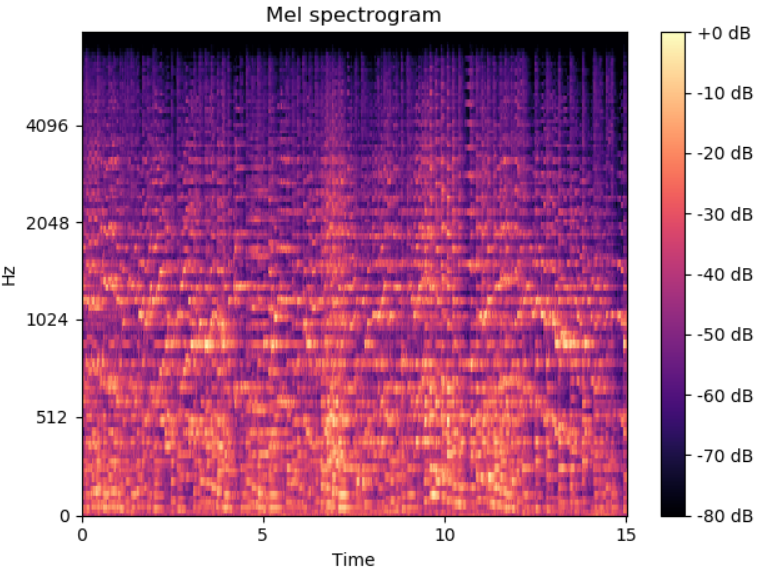
\includegraphics[scale=0.2]{./figures/classical.png}
\end{center}
\caption
{
Classical
}
\label{fig:big_picture1}
\end{figure}

\begin{figure}
\begin{center}
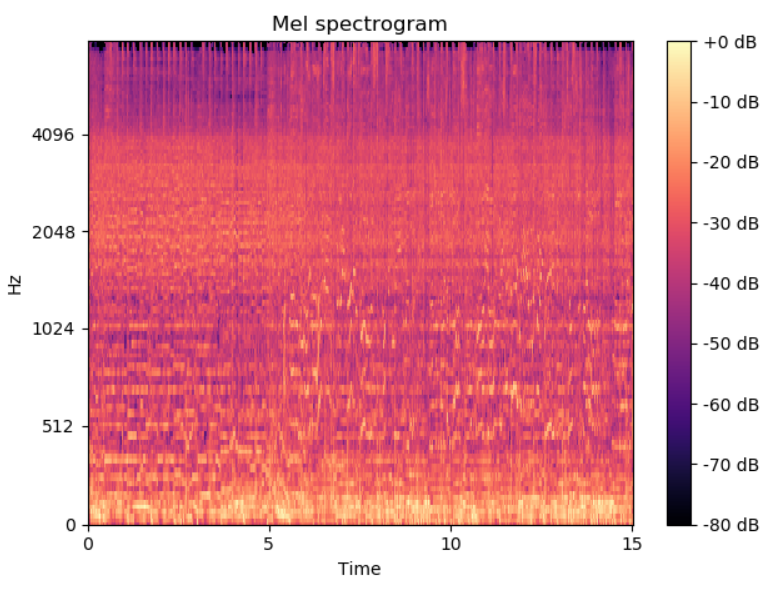
\includegraphics[scale=0.2]{./figures/metal.png}
\end{center}
\caption
{
Metal
}
\label{fig:big_picture2}
\end{figure}

\begin{figure}
\begin{center}
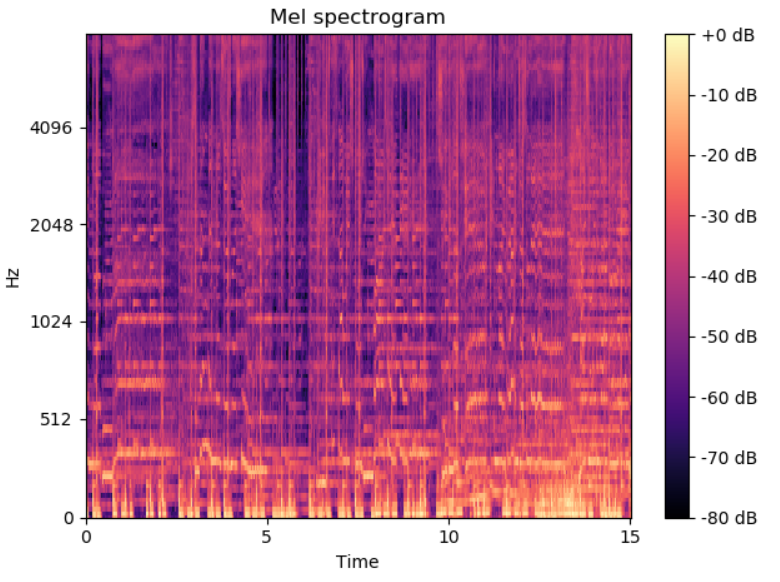
\includegraphics[scale=0.2]{./figures/pop.png}
\end{center}
\caption
{
Pop
}
\label{fig:big_picture3}
\end{figure}

\begin{figure}
\begin{center}
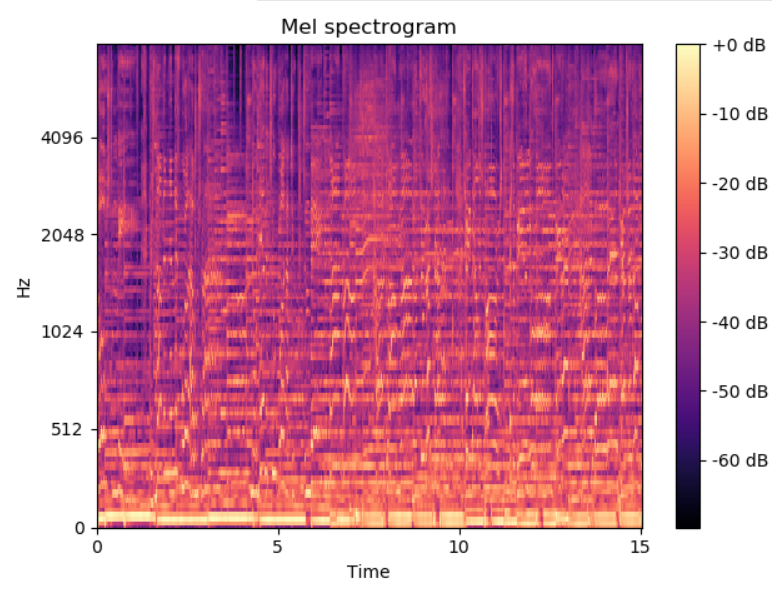
\includegraphics[scale=0.2]{./figures/country.png}
\end{center}
\caption
{
Country
}
\label{fig:big_picture4}
\end{figure}

\begin{figure}
\begin{center}
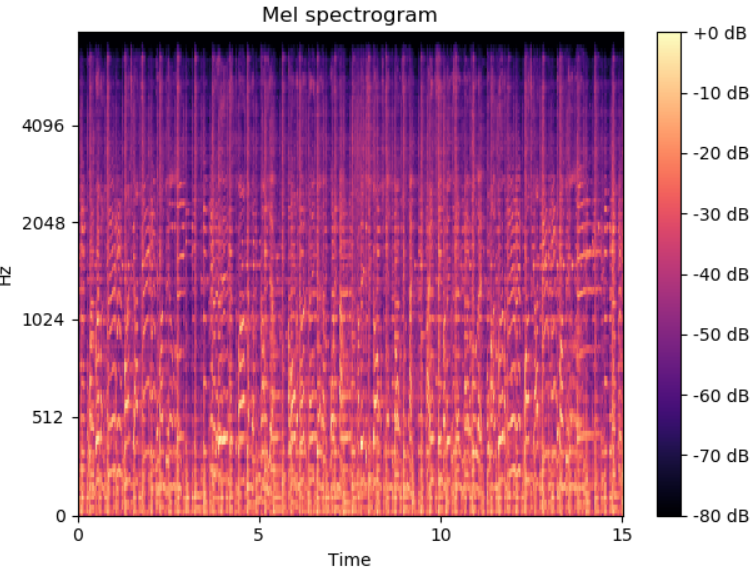
\includegraphics[scale=0.2]{./figures/blues.png}
\end{center}
\caption
{
Blues
}
\label{fig:big_picture5}
\end{figure}

\subsection{Dimensionality Reduction with Principal Component Analysis (PCA)}
After feature extraction and construction of final dataset, we thought of using dimensionality reduction before putting out data through classifiers. Since Principal Component Analysis (PCA) is a well-known and effective method for reduction of dimensions, we used PCA on our dataset. A realistic choice for number of reduced dimensions is to visualize the data with different PCA values and then pick the minimum dimension that can keep at least 95\% of the significant components. The visualization of our data with respect to different PCA dimensions and the corresponding eigenvectors is shown on Figure 6. Note that figures 7 and 8 also present a visualization of each genre in 2 and 3 dimensions. After extensive analysis of the visualization, we reduced the dimensionality to 16. Even though 16 dimensions performed very well on classifiers such as k-NN or SVM, we had to use much bigger dimensions for our neural network, since neural networks need much more data in practice. 

% Figure 6 --> PCA vs. Eigenvecs

% Figure 7 --> 2-dimensional plt 
\begin{figure}
\begin{center}
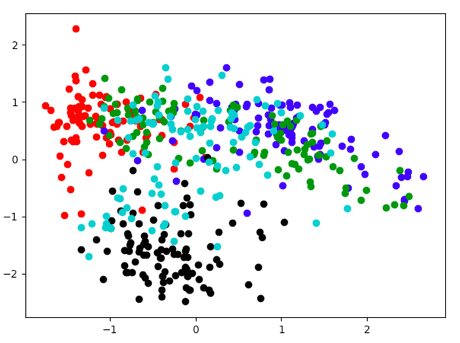
\includegraphics[scale=0.3]{./figures/2_d_plot.png}
\end{center}
\caption
{
2-d pca
}
\label{fig:big_picture5}
\end{figure}
% Figure 8 --> 3-dimensional plt 

\begin{figure}
\begin{center}
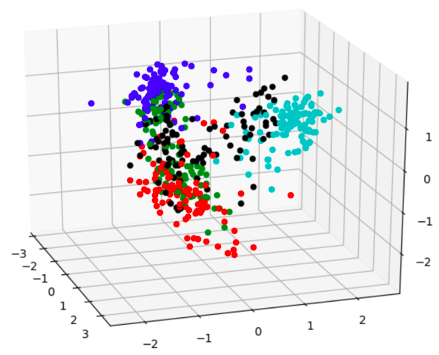
\includegraphics[scale=0.3]{./figures/3_d_plot.png}
\end{center}
\caption
{
3-d pca
}
\label{fig:big_picture5}
\end{figure}

\subsection{Machine Learning Algorithms}
\subsubsection{\textbf{K-Nearest Neighbor (K-NN)}}
The first algorithm we used is the very famous and effective k-closest neighbors algorithm. k-NN is a non-linear algorithm that can detect direct or indirect spread of data. It is very effective for huge amounts of data. The only downside of k-NN is the fact that it makes hard decisions and might produce low classification accuracy. The most significant computation in this algorithm is measuring the distance between different points in our dataset. We used Euclidean distance for k-NN, which produced good results. After our experiments, we also found that k=5 produced the best results. 

\subsubsection{\textbf{Support Vector Machines (SVM)}}
The second technique we used is the support vector machine (SVM), which is a directed organization method that discovers the extreme boundary splitting two classes of information \cite{SVM:2006}. 

\subsubsection{\textbf{Gaussian Mixture Models (GMM)}}

\subsubsection{\textbf{K-Means Clustering}}

\subsubsection{\textbf{Simple 3-layer Neural Network}}

\subsubsection{\textbf{Convolutional Neural Network (CNN)}}

\subsubsection{\textbf{Super-Classifier (SC)}}

\section{Experimental Results}\label{sec:results}

\subsection{Experiment Setup}
The experimental setup for computation of classification accuracies were quite simple. After extracting features of our data through MFCC and applying PCA, we saved our training and testing datasets into a file, so that we do not have to do all the computations again. Then, we wrote a script that loads the training and testing datasets, and then puts the training data as an input to each of our classifiers with the corresponding genre labels. After training on each classifier, we computed predictions of each song and compared each label with its groun truth. Finally, we outputted the classification accuracy of each classifier and their confusion matrices, which are shown in Figure 9 through 16.

\subsection{Classification Accuracy}

\section{Conclusion}\label{sec:conclusion}
@@@@@@@@@@@@@@@@@@@@@@@@@@@
%\section{Future Work}\label{sec:future_work}






\begin{table}
\begin{center}
\caption
{
Individual instruction type rankings are presented where the first instruction type is the most significant type for Silent Data Corruption (or crash). The ranking values next to the instruction types should be considered for computing the instruction criticality. Instruction types that are not listed are treated as the least significant ranking. 
} 
\begin{tabular}{ p{2.5cm} p{2.5cm}}
 \textbf{Crash Rank}& \textbf{SDC Rank} \\
 \hline
 1. \emph{allocate} & 8. \emph{load} \\
 2. \emph{getelementptr} & 7. \emph{add/mul}  \\
 3. \emph{load} & 6. \emph{call}  \\
 4. \emph{add/mul} & 5. \emph{allocate}  \\
 5. \emph{call} & 4. \emph{br/icmp}  \\
 6. \emph{br/icmp} & 3. \emph{getelementptr}  \\
 7. \emph{ret} & 2. \emph{store} \\
 8. \emph{store} & 1. \emph{ret}  \\
\end{tabular}
\end{center}
\end{table}

\section{Experimental Evaluation}\label{sec:evaluation}

\subsection{Setup}
We tested our reliable code generation algorithm on different benchmarks from Media Bench \cite{MediaBench:1997} and MiBench \cite{MiBench:2001}. The set of benchmark codes used in our experiments are given in Table 2. The third column of this table explains the functionality implemented by each benchmark. The next two columns give the number of basic blocks and code size in kilobytes, respectively. The last column gives the dynamic nymber of instructions executed. 

We collected statistics for a number of different applications in each benchmark and compared the SDC and Crash rates with non-modified source codes. After implementing our code generation algorithm, we again used LLFI \cite{LLFI:2015} on different benchmark applications where we first injected faults in a random manner without any modification. Then, for different overhead limits and different $\alpha$ values, we injected faults similarly to our proposed approach. In order to get accurate results, at least a thousand fault injections were conducted on the source code using a random number generator. All experiments are repeated multiple times and the average values of those experiments were reported. 

For each benchmark code in our experimental suite, we performed experiments with 3 different versions, which can be summarized as follows.\\
1)\emph{BASE}: The base execution does not employ any optimization where we injected randomized faults into unmodified LLVM IR code and collected data. \\
2)\emph{ICBR}: This is our instruction criticality based reliability (ICBR) enhancement approach where we applied our reliable code generation algorithm and collected both SDC and Crash results. \\
3)\emph{FTP}: Finally, we conducted fault injection experiments on fully tolerant and protected (FTP) programs so that we could see how close we are to a fully fault-tolerant system with a given $\alpha$ and overhead.\\

Finally, Table 3 lists the base simulation parameters used in our experiments. Unless stated otherwise, our results are collected using these parameters. We use $\alpha$ as 0.5 for the default value since we want to keep the significance of SDC and Crash the same. Note that this value can easily be changed by the user. We also set the overhead limit as 70\% to compare and prove the usefulness of our formula. Finally, we use 0.55 as the default value for DDC after our analysis and normalization of our IC formula. 


\begin{table}
\begin{center}
\caption{Benchmarks used in our experiments and their characteristics.} 
\begin{tabular}{ p{1.2cm} p{2.2cm} p{2.2cm} p{1cm} p{0.5cm} p{0.6cm} }
 Benchmark& Source & Type & Number of Basic Blocks& Code Size (KB)& Instr Count (mil)\\
 \hline
 btcnt& MiBench \cite{MiBench:2001} & Automative &  138 &  98 &  688.3 \\
 btstrng& MiBench \cite{MiBench:2001} & Automative&  56 &  48.9 &  327.3 \\
 FFT& MiBench \cite{MiBench:2001} & Telecomm & 44 & 69.2 & 238.89 \\
 qsort& MiBench \cite{MiBench:2001} & Automative & 78 &  72.3 &  513.8 \\
 adpcm& MediaBench \cite{MediaBench:1997} & Compression & 22 & 8 & 1.2\\
 gsm& MediaBench \cite{MediaBench:1997} & Telecomm & 98  &  438   &  7.09  \\
 jpeg& MediaBench \cite{MediaBench:1997} & Decompression &  112  &  488.8  &  18.65  \\
 rasta& MediaBench \cite{MediaBench:1997} & Feature Extraction &  189  &   269  &  24.86   \\
\end{tabular}
\end{center}
\end{table}
